\documentclass[twoside]{book}

% Packages required by doxygen
\usepackage{calc}
\usepackage{doxygen}
\usepackage{graphicx}
\usepackage[utf8]{inputenc}
\usepackage{makeidx}
\usepackage{multicol}
\usepackage{multirow}
\usepackage{textcomp}
\usepackage[table]{xcolor}

% Font selection
\usepackage[T1]{fontenc}
\usepackage{mathptmx}
\usepackage[scaled=.90]{helvet}
\usepackage{courier}
\usepackage{amssymb}
\usepackage{sectsty}
\renewcommand{\familydefault}{\sfdefault}
\allsectionsfont{%
  \fontseries{bc}\selectfont%
  \color{darkgray}%
}
\renewcommand{\DoxyLabelFont}{%
  \fontseries{bc}\selectfont%
  \color{darkgray}%
}

% Page & text layout
\usepackage{geometry}
\geometry{%
  a4paper,%
  top=2.5cm,%
  bottom=2.5cm,%
  left=2.5cm,%
  right=2.5cm%
}
\tolerance=750
\hfuzz=15pt
\hbadness=750
\setlength{\emergencystretch}{15pt}
\setlength{\parindent}{0cm}
\setlength{\parskip}{0.2cm}
\makeatletter
\renewcommand{\paragraph}{%
  \@startsection{paragraph}{4}{0ex}{-1.0ex}{1.0ex}{%
    \normalfont\normalsize\bfseries\SS@parafont%
  }%
}
\renewcommand{\subparagraph}{%
  \@startsection{subparagraph}{5}{0ex}{-1.0ex}{1.0ex}{%
    \normalfont\normalsize\bfseries\SS@subparafont%
  }%
}
\makeatother

% Headers & footers
\usepackage{fancyhdr}
\pagestyle{fancyplain}
\fancyhead[LE]{\fancyplain{}{\bfseries\thepage}}
\fancyhead[CE]{\fancyplain{}{}}
\fancyhead[RE]{\fancyplain{}{\bfseries\leftmark}}
\fancyhead[LO]{\fancyplain{}{\bfseries\rightmark}}
\fancyhead[CO]{\fancyplain{}{}}
\fancyhead[RO]{\fancyplain{}{\bfseries\thepage}}
\fancyfoot[LE]{\fancyplain{}{}}
\fancyfoot[CE]{\fancyplain{}{}}
\fancyfoot[RE]{\fancyplain{}{\bfseries\scriptsize Generated on Tue Apr 28 2015 17\-:22\-:42 for My Project by Doxygen }}
\fancyfoot[LO]{\fancyplain{}{\bfseries\scriptsize Generated on Tue Apr 28 2015 17\-:22\-:42 for My Project by Doxygen }}
\fancyfoot[CO]{\fancyplain{}{}}
\fancyfoot[RO]{\fancyplain{}{}}
\renewcommand{\footrulewidth}{0.4pt}
\renewcommand{\chaptermark}[1]{%
  \markboth{#1}{}%
}
\renewcommand{\sectionmark}[1]{%
  \markright{\thesection\ #1}%
}

% Indices & bibliography
\usepackage{natbib}
\usepackage[titles]{tocloft}
\setcounter{tocdepth}{3}
\setcounter{secnumdepth}{5}
\makeindex

% Hyperlinks (required, but should be loaded last)
\usepackage{ifpdf}
\ifpdf
  \usepackage[pdftex,pagebackref=true]{hyperref}
\else
  \usepackage[ps2pdf,pagebackref=true]{hyperref}
\fi
\hypersetup{%
  colorlinks=true,%
  linkcolor=blue,%
  citecolor=blue,%
  unicode%
}

% Custom commands
\newcommand{\clearemptydoublepage}{%
  \newpage{\pagestyle{empty}\cleardoublepage}%
}


%===== C O N T E N T S =====

\begin{document}

% Titlepage & ToC
\hypersetup{pageanchor=false}
\pagenumbering{roman}
\begin{titlepage}
\vspace*{7cm}
\begin{center}%
{\Large My Project }\\
\vspace*{1cm}
{\large Generated by Doxygen 1.8.5}\\
\vspace*{0.5cm}
{\small Tue Apr 28 2015 17:22:42}\\
\end{center}
\end{titlepage}
\clearemptydoublepage
\tableofcontents
\clearemptydoublepage
\pagenumbering{arabic}
\hypersetup{pageanchor=true}

%--- Begin generated contents ---
\chapter{Hierarchical Index}
\section{Class Hierarchy}
This inheritance list is sorted roughly, but not completely, alphabetically\-:\begin{DoxyCompactList}
\item \contentsline{section}{com.\-deltafountains.\-Joy\-Stick\-Class}{\pageref{classcom_1_1deltafountains_1_1JoyStickClass}}{}
\item Activity\begin{DoxyCompactList}
\item \contentsline{section}{com.\-deltafountains.\-Controls}{\pageref{classcom_1_1deltafountains_1_1Controls}}{}
\item \contentsline{section}{com.\-deltafountains.\-Functions}{\pageref{classcom_1_1deltafountains_1_1Functions}}{}
\item \contentsline{section}{com.\-deltafountains.\-Main\-Activity}{\pageref{classcom_1_1deltafountains_1_1MainActivity}}{}
\item \contentsline{section}{com.\-deltafountains.\-Settings}{\pageref{classcom_1_1deltafountains_1_1Settings}}{}
\item \contentsline{section}{com.\-deltafountains.\-Support}{\pageref{classcom_1_1deltafountains_1_1Support}}{}
\end{DoxyCompactList}
\end{DoxyCompactList}

\chapter{Class Index}
\section{Class List}
Here are the classes, structs, unions and interfaces with brief descriptions\-:\begin{DoxyCompactList}
\item\contentsline{section}{\hyperlink{classcom_1_1deltafountains_1_1Controls}{com.\-deltafountains.\-Controls} }{\pageref{classcom_1_1deltafountains_1_1Controls}}{}
\item\contentsline{section}{\hyperlink{classcom_1_1deltafountains_1_1Functions}{com.\-deltafountains.\-Functions} }{\pageref{classcom_1_1deltafountains_1_1Functions}}{}
\item\contentsline{section}{\hyperlink{classcom_1_1deltafountains_1_1JoyStickClass}{com.\-deltafountains.\-Joy\-Stick\-Class} }{\pageref{classcom_1_1deltafountains_1_1JoyStickClass}}{}
\item\contentsline{section}{\hyperlink{classcom_1_1deltafountains_1_1MainActivity}{com.\-deltafountains.\-Main\-Activity} }{\pageref{classcom_1_1deltafountains_1_1MainActivity}}{}
\item\contentsline{section}{\hyperlink{classcom_1_1deltafountains_1_1Settings}{com.\-deltafountains.\-Settings} }{\pageref{classcom_1_1deltafountains_1_1Settings}}{}
\item\contentsline{section}{\hyperlink{classcom_1_1deltafountains_1_1Support}{com.\-deltafountains.\-Support} }{\pageref{classcom_1_1deltafountains_1_1Support}}{}
\end{DoxyCompactList}

\chapter{Class Documentation}
\hypertarget{classcom_1_1deltafountains_1_1Controls}{\section{com.\-deltafountains.\-Controls Class Reference}
\label{classcom_1_1deltafountains_1_1Controls}\index{com.\-deltafountains.\-Controls@{com.\-deltafountains.\-Controls}}
}
Inheritance diagram for com.\-deltafountains.\-Controls\-:\begin{figure}[H]
\begin{center}
\leavevmode
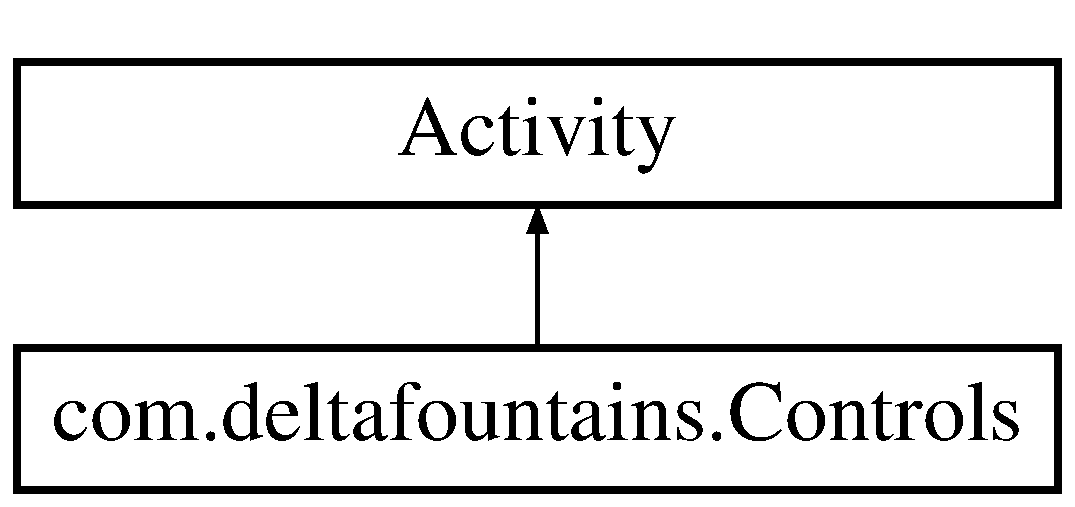
\includegraphics[height=2.000000cm]{classcom_1_1deltafountains_1_1Controls}
\end{center}
\end{figure}
\subsection*{Classes}
\begin{DoxyCompactItemize}
\item 
class {\bfseries Client\-Thread}
\end{DoxyCompactItemize}
\subsection*{Public Member Functions}
\begin{DoxyCompactItemize}
\item 
\hypertarget{classcom_1_1deltafountains_1_1Controls_a5bdfda504eff84fd5726b7379a1bd062}{void {\bfseries on\-Create} (Bundle saved\-Instance\-State)}\label{classcom_1_1deltafountains_1_1Controls_a5bdfda504eff84fd5726b7379a1bd062}

\item 
\hypertarget{classcom_1_1deltafountains_1_1Controls_a45b720712d8a6d35270828b46828a9aa}{boolean {\bfseries on\-Options\-Item\-Selected} (Menu\-Item item)}\label{classcom_1_1deltafountains_1_1Controls_a45b720712d8a6d35270828b46828a9aa}

\end{DoxyCompactItemize}


The documentation for this class was generated from the following file\-:\begin{DoxyCompactItemize}
\item 
Controls.\-java\end{DoxyCompactItemize}

\hypertarget{classcom_1_1deltafountains_1_1Functions}{\section{com.\-deltafountains.\-Functions Class Reference}
\label{classcom_1_1deltafountains_1_1Functions}\index{com.\-deltafountains.\-Functions@{com.\-deltafountains.\-Functions}}
}
Inheritance diagram for com.\-deltafountains.\-Functions\-:\begin{figure}[H]
\begin{center}
\leavevmode
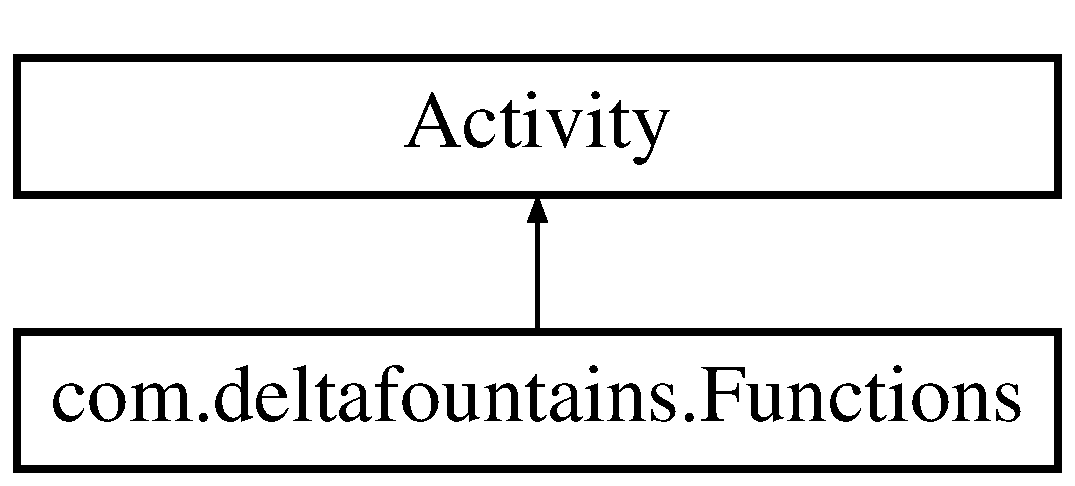
\includegraphics[height=2.000000cm]{classcom_1_1deltafountains_1_1Functions}
\end{center}
\end{figure}
\subsection*{Classes}
\begin{DoxyCompactItemize}
\item 
class {\bfseries Client\-Thread}
\end{DoxyCompactItemize}
\subsection*{Public Member Functions}
\begin{DoxyCompactItemize}
\item 
\hypertarget{classcom_1_1deltafountains_1_1Functions_a39dce752a9e7bea4e975352020e7b44f}{boolean {\bfseries on\-Options\-Item\-Selected} (Menu\-Item item)}\label{classcom_1_1deltafountains_1_1Functions_a39dce752a9e7bea4e975352020e7b44f}

\end{DoxyCompactItemize}
\subsection*{Protected Member Functions}
\begin{DoxyCompactItemize}
\item 
\hypertarget{classcom_1_1deltafountains_1_1Functions_a3660032f995c222019bfa8e15ed0ea62}{void {\bfseries on\-Create} (Bundle saved\-Instance\-State)}\label{classcom_1_1deltafountains_1_1Functions_a3660032f995c222019bfa8e15ed0ea62}

\end{DoxyCompactItemize}


The documentation for this class was generated from the following file\-:\begin{DoxyCompactItemize}
\item 
Functions.\-java\end{DoxyCompactItemize}

\hypertarget{classcom_1_1deltafountains_1_1JoyStickClass}{\section{com.\-deltafountains.\-Joy\-Stick\-Class Class Reference}
\label{classcom_1_1deltafountains_1_1JoyStickClass}\index{com.\-deltafountains.\-Joy\-Stick\-Class@{com.\-deltafountains.\-Joy\-Stick\-Class}}
}
\subsection*{Public Member Functions}
\begin{DoxyCompactItemize}
\item 
\hypertarget{classcom_1_1deltafountains_1_1JoyStickClass_abba638ed88b4dd43c9132af7baeec361}{{\bfseries Joy\-Stick\-Class} (Context context, View\-Group layout, int stick\-\_\-res\-\_\-id)}\label{classcom_1_1deltafountains_1_1JoyStickClass_abba638ed88b4dd43c9132af7baeec361}

\item 
\hypertarget{classcom_1_1deltafountains_1_1JoyStickClass_a09027d634492c7baae36d50c5ce7464a}{void {\bfseries draw\-Stick} (Motion\-Event arg1)}\label{classcom_1_1deltafountains_1_1JoyStickClass_a09027d634492c7baae36d50c5ce7464a}

\item 
\hypertarget{classcom_1_1deltafountains_1_1JoyStickClass_adc92209cddd918b2b3ab601d0ed51c9f}{int\mbox{[}$\,$\mbox{]} {\bfseries get\-Position} ()}\label{classcom_1_1deltafountains_1_1JoyStickClass_adc92209cddd918b2b3ab601d0ed51c9f}

\item 
\hypertarget{classcom_1_1deltafountains_1_1JoyStickClass_a7ac1c79facfa6fd4d9b4eb1eafba47a9}{int {\bfseries get\-X} ()}\label{classcom_1_1deltafountains_1_1JoyStickClass_a7ac1c79facfa6fd4d9b4eb1eafba47a9}

\item 
\hypertarget{classcom_1_1deltafountains_1_1JoyStickClass_aeee0012998434297d88cdc23b4461953}{int {\bfseries get\-Y} ()}\label{classcom_1_1deltafountains_1_1JoyStickClass_aeee0012998434297d88cdc23b4461953}

\item 
\hypertarget{classcom_1_1deltafountains_1_1JoyStickClass_a76f2418adec095443d59ba8f88a43f29}{float {\bfseries get\-Angle} ()}\label{classcom_1_1deltafountains_1_1JoyStickClass_a76f2418adec095443d59ba8f88a43f29}

\item 
\hypertarget{classcom_1_1deltafountains_1_1JoyStickClass_a453d64dfea113ef628867be3a89f37fe}{float {\bfseries get\-Distance} ()}\label{classcom_1_1deltafountains_1_1JoyStickClass_a453d64dfea113ef628867be3a89f37fe}

\item 
\hypertarget{classcom_1_1deltafountains_1_1JoyStickClass_a00011a3ab853263103851b196da0ceeb}{void {\bfseries set\-Minimum\-Distance} (int min\-Distance)}\label{classcom_1_1deltafountains_1_1JoyStickClass_a00011a3ab853263103851b196da0ceeb}

\item 
\hypertarget{classcom_1_1deltafountains_1_1JoyStickClass_abd27213abdd967bd78cdb94e65723127}{int {\bfseries get\-Minimum\-Distance} ()}\label{classcom_1_1deltafountains_1_1JoyStickClass_abd27213abdd967bd78cdb94e65723127}

\item 
\hypertarget{classcom_1_1deltafountains_1_1JoyStickClass_a99641c0c263787ff8059d55c417e6a7a}{int {\bfseries get8\-Direction} ()}\label{classcom_1_1deltafountains_1_1JoyStickClass_a99641c0c263787ff8059d55c417e6a7a}

\item 
\hypertarget{classcom_1_1deltafountains_1_1JoyStickClass_a9123113bfa59c118f4a8360592a4c425}{int {\bfseries get4\-Direction} ()}\label{classcom_1_1deltafountains_1_1JoyStickClass_a9123113bfa59c118f4a8360592a4c425}

\item 
\hypertarget{classcom_1_1deltafountains_1_1JoyStickClass_a385ab325cf05bb8c12ae0e15058e233a}{void {\bfseries set\-Offset} (int offset)}\label{classcom_1_1deltafountains_1_1JoyStickClass_a385ab325cf05bb8c12ae0e15058e233a}

\item 
\hypertarget{classcom_1_1deltafountains_1_1JoyStickClass_af7cfb4ffa955a74608b41122f74ebdd8}{int {\bfseries get\-Offset} ()}\label{classcom_1_1deltafountains_1_1JoyStickClass_af7cfb4ffa955a74608b41122f74ebdd8}

\item 
\hypertarget{classcom_1_1deltafountains_1_1JoyStickClass_aaa83a7db1f989a3ef52c7877b7bfa714}{void {\bfseries set\-Stick\-Alpha} (int alpha)}\label{classcom_1_1deltafountains_1_1JoyStickClass_aaa83a7db1f989a3ef52c7877b7bfa714}

\item 
\hypertarget{classcom_1_1deltafountains_1_1JoyStickClass_a5bf2ec0f06ecbd3b05685ae021af04fb}{int {\bfseries get\-Stick\-Alpha} ()}\label{classcom_1_1deltafountains_1_1JoyStickClass_a5bf2ec0f06ecbd3b05685ae021af04fb}

\item 
\hypertarget{classcom_1_1deltafountains_1_1JoyStickClass_a15ecdb0bc38cc5b08f9b4b7a0c1863ea}{void {\bfseries set\-Layout\-Alpha} (int alpha)}\label{classcom_1_1deltafountains_1_1JoyStickClass_a15ecdb0bc38cc5b08f9b4b7a0c1863ea}

\item 
\hypertarget{classcom_1_1deltafountains_1_1JoyStickClass_a8e09cba9a571f0efd4560c4500a94c1f}{int {\bfseries get\-Layout\-Alpha} ()}\label{classcom_1_1deltafountains_1_1JoyStickClass_a8e09cba9a571f0efd4560c4500a94c1f}

\item 
\hypertarget{classcom_1_1deltafountains_1_1JoyStickClass_a2aee2574551a71f6ed4794c08b721c71}{void {\bfseries set\-Stick\-Size} (int width, int height)}\label{classcom_1_1deltafountains_1_1JoyStickClass_a2aee2574551a71f6ed4794c08b721c71}

\item 
\hypertarget{classcom_1_1deltafountains_1_1JoyStickClass_a308b46d6391f7e946333c0755288cabf}{void {\bfseries set\-Stick\-Width} (int width)}\label{classcom_1_1deltafountains_1_1JoyStickClass_a308b46d6391f7e946333c0755288cabf}

\item 
\hypertarget{classcom_1_1deltafountains_1_1JoyStickClass_aba5fd3513e05fb5bbaa68854f925ccd6}{void {\bfseries set\-Stick\-Height} (int height)}\label{classcom_1_1deltafountains_1_1JoyStickClass_aba5fd3513e05fb5bbaa68854f925ccd6}

\item 
\hypertarget{classcom_1_1deltafountains_1_1JoyStickClass_a69e6b81c8321d339a52e87443ff5fc34}{int {\bfseries get\-Stick\-Width} ()}\label{classcom_1_1deltafountains_1_1JoyStickClass_a69e6b81c8321d339a52e87443ff5fc34}

\item 
\hypertarget{classcom_1_1deltafountains_1_1JoyStickClass_a38fa053bfb1621ecfa57f5c6cce95626}{int {\bfseries get\-Stick\-Height} ()}\label{classcom_1_1deltafountains_1_1JoyStickClass_a38fa053bfb1621ecfa57f5c6cce95626}

\item 
\hypertarget{classcom_1_1deltafountains_1_1JoyStickClass_ac923913d15364dd7f99623c7d669585b}{void {\bfseries set\-Layout\-Size} (int width, int height)}\label{classcom_1_1deltafountains_1_1JoyStickClass_ac923913d15364dd7f99623c7d669585b}

\item 
\hypertarget{classcom_1_1deltafountains_1_1JoyStickClass_a294660f8601beedcfb17936358c4f2ea}{int {\bfseries get\-Layout\-Width} ()}\label{classcom_1_1deltafountains_1_1JoyStickClass_a294660f8601beedcfb17936358c4f2ea}

\item 
\hypertarget{classcom_1_1deltafountains_1_1JoyStickClass_aacda01cc49eecc56681aad9a7489617f}{int {\bfseries get\-Layout\-Height} ()}\label{classcom_1_1deltafountains_1_1JoyStickClass_aacda01cc49eecc56681aad9a7489617f}

\end{DoxyCompactItemize}
\subsection*{Static Public Attributes}
\begin{DoxyCompactItemize}
\item 
\hypertarget{classcom_1_1deltafountains_1_1JoyStickClass_a7754b0ec4eea08c1f6c976dc26e99b59}{static final int {\bfseries S\-T\-I\-C\-K\-\_\-\-N\-O\-N\-E} = 0}\label{classcom_1_1deltafountains_1_1JoyStickClass_a7754b0ec4eea08c1f6c976dc26e99b59}

\item 
\hypertarget{classcom_1_1deltafountains_1_1JoyStickClass_a7cdda747bf39f1a02f103d3abb418d42}{static final int {\bfseries S\-T\-I\-C\-K\-\_\-\-U\-P} = 1}\label{classcom_1_1deltafountains_1_1JoyStickClass_a7cdda747bf39f1a02f103d3abb418d42}

\item 
\hypertarget{classcom_1_1deltafountains_1_1JoyStickClass_a2bd33722100c50c2462830c83abec3c1}{static final int {\bfseries S\-T\-I\-C\-K\-\_\-\-U\-P\-R\-I\-G\-H\-T} = 2}\label{classcom_1_1deltafountains_1_1JoyStickClass_a2bd33722100c50c2462830c83abec3c1}

\item 
\hypertarget{classcom_1_1deltafountains_1_1JoyStickClass_a8952bbe3a7c01722cde45924bf3416d2}{static final int {\bfseries S\-T\-I\-C\-K\-\_\-\-R\-I\-G\-H\-T} = 3}\label{classcom_1_1deltafountains_1_1JoyStickClass_a8952bbe3a7c01722cde45924bf3416d2}

\item 
\hypertarget{classcom_1_1deltafountains_1_1JoyStickClass_a4d4b66fa1de0ee52aa5dcb31acd290eb}{static final int {\bfseries S\-T\-I\-C\-K\-\_\-\-D\-O\-W\-N\-R\-I\-G\-H\-T} = 4}\label{classcom_1_1deltafountains_1_1JoyStickClass_a4d4b66fa1de0ee52aa5dcb31acd290eb}

\item 
\hypertarget{classcom_1_1deltafountains_1_1JoyStickClass_a678b1466c665e03dbe8c7dbe07672dd4}{static final int {\bfseries S\-T\-I\-C\-K\-\_\-\-D\-O\-W\-N} = 5}\label{classcom_1_1deltafountains_1_1JoyStickClass_a678b1466c665e03dbe8c7dbe07672dd4}

\item 
\hypertarget{classcom_1_1deltafountains_1_1JoyStickClass_a45dd55e2e1d991c7b094e1fb37203d00}{static final int {\bfseries S\-T\-I\-C\-K\-\_\-\-D\-O\-W\-N\-L\-E\-F\-T} = 6}\label{classcom_1_1deltafountains_1_1JoyStickClass_a45dd55e2e1d991c7b094e1fb37203d00}

\item 
\hypertarget{classcom_1_1deltafountains_1_1JoyStickClass_afa3af1ec91521e7e9a7ac393a75d997e}{static final int {\bfseries S\-T\-I\-C\-K\-\_\-\-L\-E\-F\-T} = 7}\label{classcom_1_1deltafountains_1_1JoyStickClass_afa3af1ec91521e7e9a7ac393a75d997e}

\item 
\hypertarget{classcom_1_1deltafountains_1_1JoyStickClass_a365728f3e509df6e57857214b5131eaf}{static final int {\bfseries S\-T\-I\-C\-K\-\_\-\-U\-P\-L\-E\-F\-T} = 8}\label{classcom_1_1deltafountains_1_1JoyStickClass_a365728f3e509df6e57857214b5131eaf}

\end{DoxyCompactItemize}


The documentation for this class was generated from the following file\-:\begin{DoxyCompactItemize}
\item 
Joy\-Stick\-Class.\-java\end{DoxyCompactItemize}

\hypertarget{classcom_1_1deltafountains_1_1MainActivity}{\section{com.\-deltafountains.\-Main\-Activity Class Reference}
\label{classcom_1_1deltafountains_1_1MainActivity}\index{com.\-deltafountains.\-Main\-Activity@{com.\-deltafountains.\-Main\-Activity}}
}
Inheritance diagram for com.\-deltafountains.\-Main\-Activity\-:\begin{figure}[H]
\begin{center}
\leavevmode
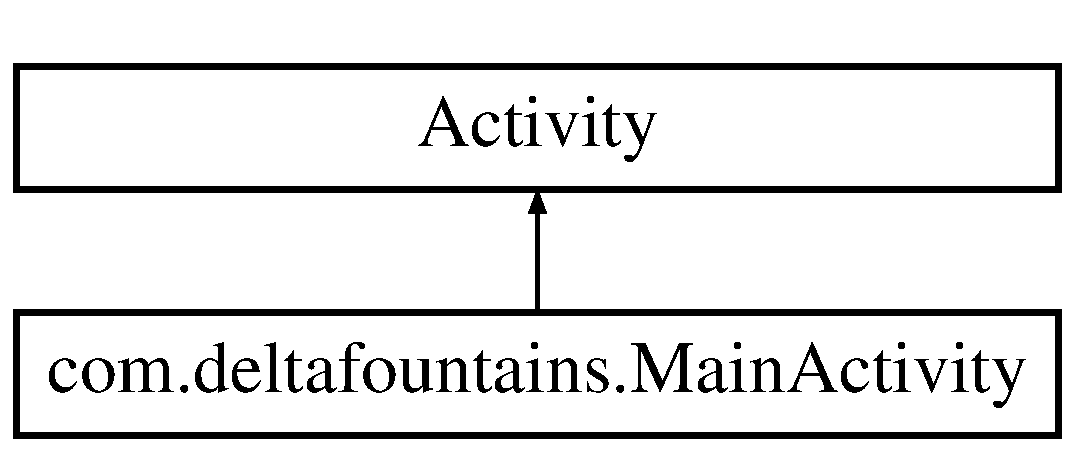
\includegraphics[height=2.000000cm]{classcom_1_1deltafountains_1_1MainActivity}
\end{center}
\end{figure}
\subsection*{Public Member Functions}
\begin{DoxyCompactItemize}
\item 
\hypertarget{classcom_1_1deltafountains_1_1MainActivity_aafda8d017f103f7f31a97a0029a7cacc}{boolean {\bfseries on\-Options\-Item\-Selected} (Menu\-Item item)}\label{classcom_1_1deltafountains_1_1MainActivity_aafda8d017f103f7f31a97a0029a7cacc}

\end{DoxyCompactItemize}
\subsection*{Protected Member Functions}
\begin{DoxyCompactItemize}
\item 
\hypertarget{classcom_1_1deltafountains_1_1MainActivity_aaf458bbf1f883307df234bdda5e368f4}{void {\bfseries on\-Create} (Bundle saved\-Instance\-State)}\label{classcom_1_1deltafountains_1_1MainActivity_aaf458bbf1f883307df234bdda5e368f4}

\end{DoxyCompactItemize}


The documentation for this class was generated from the following file\-:\begin{DoxyCompactItemize}
\item 
Main\-Activity.\-java\end{DoxyCompactItemize}

\hypertarget{classcom_1_1deltafountains_1_1Settings}{\section{com.\-deltafountains.\-Settings Class Reference}
\label{classcom_1_1deltafountains_1_1Settings}\index{com.\-deltafountains.\-Settings@{com.\-deltafountains.\-Settings}}
}
Inheritance diagram for com.\-deltafountains.\-Settings\-:\begin{figure}[H]
\begin{center}
\leavevmode
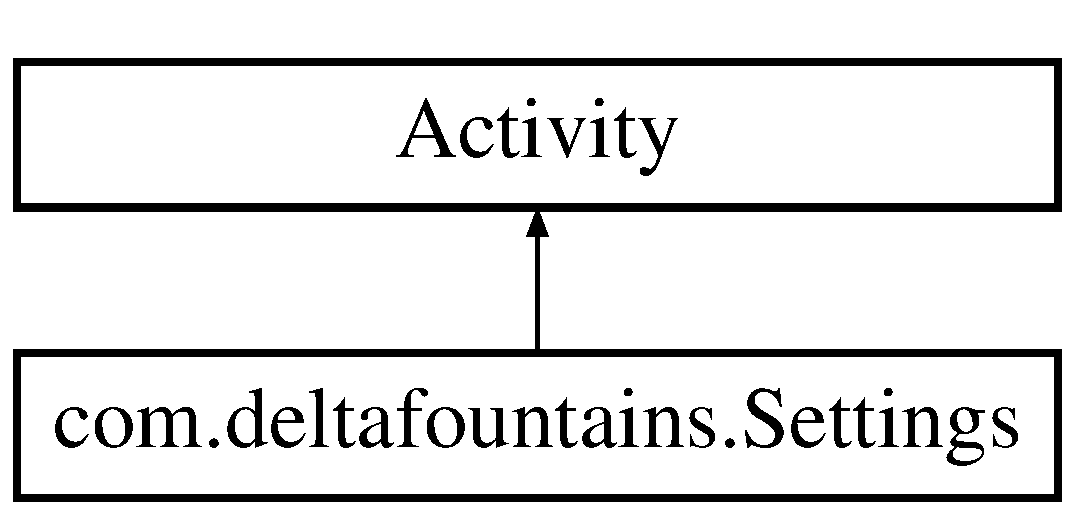
\includegraphics[height=2.000000cm]{classcom_1_1deltafountains_1_1Settings}
\end{center}
\end{figure}
\subsection*{Public Member Functions}
\begin{DoxyCompactItemize}
\item 
\hypertarget{classcom_1_1deltafountains_1_1Settings_a98bf9b724b8e96b61e0f9488ec041222}{boolean {\bfseries on\-Options\-Item\-Selected} (Menu\-Item item)}\label{classcom_1_1deltafountains_1_1Settings_a98bf9b724b8e96b61e0f9488ec041222}

\end{DoxyCompactItemize}
\subsection*{Protected Member Functions}
\begin{DoxyCompactItemize}
\item 
\hypertarget{classcom_1_1deltafountains_1_1Settings_a47b242e34f20a763ad926be34e0531bc}{void {\bfseries on\-Create} (Bundle saved\-Instance\-State)}\label{classcom_1_1deltafountains_1_1Settings_a47b242e34f20a763ad926be34e0531bc}

\end{DoxyCompactItemize}


The documentation for this class was generated from the following file\-:\begin{DoxyCompactItemize}
\item 
Settings.\-java\end{DoxyCompactItemize}

\hypertarget{classcom_1_1deltafountains_1_1Support}{\section{com.\-deltafountains.\-Support Class Reference}
\label{classcom_1_1deltafountains_1_1Support}\index{com.\-deltafountains.\-Support@{com.\-deltafountains.\-Support}}
}
Inheritance diagram for com.\-deltafountains.\-Support\-:\begin{figure}[H]
\begin{center}
\leavevmode
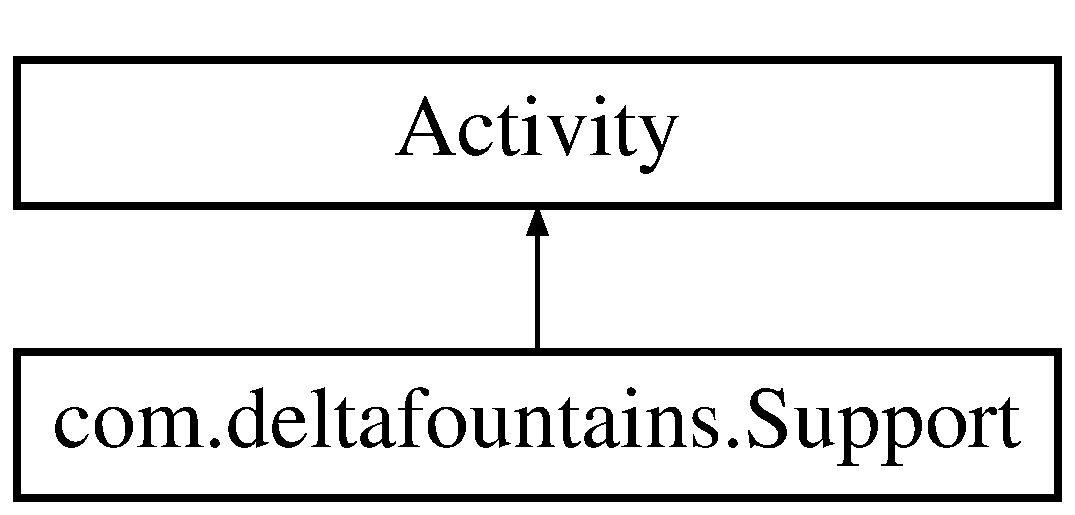
\includegraphics[height=2.000000cm]{classcom_1_1deltafountains_1_1Support}
\end{center}
\end{figure}
\subsection*{Public Member Functions}
\begin{DoxyCompactItemize}
\item 
\hypertarget{classcom_1_1deltafountains_1_1Support_ac26a3d1ea1a57b75119b729a5cd33cae}{boolean {\bfseries on\-Options\-Item\-Selected} (Menu\-Item item)}\label{classcom_1_1deltafountains_1_1Support_ac26a3d1ea1a57b75119b729a5cd33cae}

\end{DoxyCompactItemize}
\subsection*{Protected Member Functions}
\begin{DoxyCompactItemize}
\item 
\hypertarget{classcom_1_1deltafountains_1_1Support_ada4d19e2f16dea46b8973ab7cb443de5}{void {\bfseries on\-Create} (Bundle saved\-Instance\-State)}\label{classcom_1_1deltafountains_1_1Support_ada4d19e2f16dea46b8973ab7cb443de5}

\end{DoxyCompactItemize}


The documentation for this class was generated from the following file\-:\begin{DoxyCompactItemize}
\item 
Support.\-java\end{DoxyCompactItemize}

%--- End generated contents ---

% Index
\newpage
\phantomsection
\addcontentsline{toc}{part}{Index}
\printindex

\end{document}
